\documentclass[12pt]{report}

\usepackage{amsmath} % loads AMS-Math package
\usepackage{euscript}
\usepackage{amssymb}
\usepackage{epsfig} % allows PostScript files
\usepackage{graphicx}
\usepackage{multirow}
\usepackage{listings} % allows lstlisting environment
\usepackage{moreverb} % allows listinginput environment
\usepackage{vmargin} % allows better margins
\usepackage{color}
\setpapersize{USletter} % sets the paper size
\allowdisplaybreaks[1]
\setmarginsrb{1in}{0.7in}{1in}{1in}{12pt}{11mm}{0pt}{11mm} %sets margins


\title{\LaTeX \ Title }

\author{Alex Beutel  \\
{\small\em \copyright \  Draft date \today }}

 \date{ }

 %\abstract{Some bullshit}

\begin{document}

\maketitle
\begin{abstract}
	blah blah blah
\end{abstract}
 %\addcontentsline{toc}{chapter}{Contents}
\pagenumbering{roman}
\tableofcontents
\listoffigures
\listoftables

\pagestyle{headings}
\pagenumbering{arabic}

\pagestyle{plain}

\chapter{Introduction}

\input{writing/intro}

\chapter{Chaos Theory}

\chapter{Experimental Setup}

\chapter{Results}

\section{Data Analysis} % (fold)
\label{sec:Data Analysis}

% section Data Analysis (end)

\section{Error Analysis} % (fold)
\label{sec:Error Analysis}

% section Error Analysis (end)

\chapter{Simulations} % (fold)
\label{ch:Simulations}

% section Simulations (end)

	\begin{figure}[h]
		\centering
		% GNUPLOT: LaTeX picture
\setlength{\unitlength}{0.240900pt}
\ifx\plotpoint\undefined\newsavebox{\plotpoint}\fi
\sbox{\plotpoint}{\rule[-0.200pt]{0.400pt}{0.400pt}}%
\begin{picture}(1500,900)(0,0)
\sbox{\plotpoint}{\rule[-0.200pt]{0.400pt}{0.400pt}}%
\put(191.0,131.0){\rule[-0.200pt]{4.818pt}{0.400pt}}
\put(171,131){\makebox(0,0)[r]{ 50}}
\put(1429.0,131.0){\rule[-0.200pt]{4.818pt}{0.400pt}}
\put(191.0,223.0){\rule[-0.200pt]{4.818pt}{0.400pt}}
\put(171,223){\makebox(0,0)[r]{ 60}}
\put(1429.0,223.0){\rule[-0.200pt]{4.818pt}{0.400pt}}
\put(191.0,315.0){\rule[-0.200pt]{4.818pt}{0.400pt}}
\put(171,315){\makebox(0,0)[r]{ 70}}
\put(1429.0,315.0){\rule[-0.200pt]{4.818pt}{0.400pt}}
\put(191.0,407.0){\rule[-0.200pt]{4.818pt}{0.400pt}}
\put(171,407){\makebox(0,0)[r]{ 80}}
\put(1429.0,407.0){\rule[-0.200pt]{4.818pt}{0.400pt}}
\put(191.0,500.0){\rule[-0.200pt]{4.818pt}{0.400pt}}
\put(171,500){\makebox(0,0)[r]{ 90}}
\put(1429.0,500.0){\rule[-0.200pt]{4.818pt}{0.400pt}}
\put(191.0,592.0){\rule[-0.200pt]{4.818pt}{0.400pt}}
\put(171,592){\makebox(0,0)[r]{ 100}}
\put(1429.0,592.0){\rule[-0.200pt]{4.818pt}{0.400pt}}
\put(191.0,684.0){\rule[-0.200pt]{4.818pt}{0.400pt}}
\put(171,684){\makebox(0,0)[r]{ 110}}
\put(1429.0,684.0){\rule[-0.200pt]{4.818pt}{0.400pt}}
\put(191.0,776.0){\rule[-0.200pt]{4.818pt}{0.400pt}}
\put(171,776){\makebox(0,0)[r]{ 120}}
\put(1429.0,776.0){\rule[-0.200pt]{4.818pt}{0.400pt}}
\put(191.0,131.0){\rule[-0.200pt]{0.400pt}{4.818pt}}
\put(191,90){\makebox(0,0){ 14}}
\put(191.0,756.0){\rule[-0.200pt]{0.400pt}{4.818pt}}
\put(331.0,131.0){\rule[-0.200pt]{0.400pt}{4.818pt}}
\put(331,90){\makebox(0,0){ 15}}
\put(331.0,756.0){\rule[-0.200pt]{0.400pt}{4.818pt}}
\put(471.0,131.0){\rule[-0.200pt]{0.400pt}{4.818pt}}
\put(471,90){\makebox(0,0){ 16}}
\put(471.0,756.0){\rule[-0.200pt]{0.400pt}{4.818pt}}
\put(610.0,131.0){\rule[-0.200pt]{0.400pt}{4.818pt}}
\put(610,90){\makebox(0,0){ 17}}
\put(610.0,756.0){\rule[-0.200pt]{0.400pt}{4.818pt}}
\put(750.0,131.0){\rule[-0.200pt]{0.400pt}{4.818pt}}
\put(750,90){\makebox(0,0){ 18}}
\put(750.0,756.0){\rule[-0.200pt]{0.400pt}{4.818pt}}
\put(890.0,131.0){\rule[-0.200pt]{0.400pt}{4.818pt}}
\put(890,90){\makebox(0,0){ 19}}
\put(890.0,756.0){\rule[-0.200pt]{0.400pt}{4.818pt}}
\put(1030.0,131.0){\rule[-0.200pt]{0.400pt}{4.818pt}}
\put(1030,90){\makebox(0,0){ 20}}
\put(1030.0,756.0){\rule[-0.200pt]{0.400pt}{4.818pt}}
\put(1169.0,131.0){\rule[-0.200pt]{0.400pt}{4.818pt}}
\put(1169,90){\makebox(0,0){ 21}}
\put(1169.0,756.0){\rule[-0.200pt]{0.400pt}{4.818pt}}
\put(1309.0,131.0){\rule[-0.200pt]{0.400pt}{4.818pt}}
\put(1309,90){\makebox(0,0){ 22}}
\put(1309.0,756.0){\rule[-0.200pt]{0.400pt}{4.818pt}}
\put(1449.0,131.0){\rule[-0.200pt]{0.400pt}{4.818pt}}
\put(1449,90){\makebox(0,0){ 23}}
\put(1449.0,756.0){\rule[-0.200pt]{0.400pt}{4.818pt}}
\put(191.0,131.0){\rule[-0.200pt]{0.400pt}{155.380pt}}
\put(191.0,131.0){\rule[-0.200pt]{303.052pt}{0.400pt}}
\put(1449.0,131.0){\rule[-0.200pt]{0.400pt}{155.380pt}}
\put(191.0,776.0){\rule[-0.200pt]{303.052pt}{0.400pt}}
\put(50,453){\makebox(0,0){\shortstack{V$_{\rm resistor}$\\(mV)}}}
\put(820,29){\makebox(0,0){V$_{\rm drive}$ (mV)}}
\put(820,838){\makebox(0,0){Bifurcation for 100khz}}
\put(261,182){\rule{1pt}{1pt}}
\put(317,205){\rule{1pt}{1pt}}
\put(373,214){\rule{1pt}{1pt}}
\put(429,237){\rule{1pt}{1pt}}
\put(429,196){\rule{1pt}{1pt}}
\put(485,265){\rule{1pt}{1pt}}
\put(485,177){\rule{1pt}{1pt}}
\put(568,301){\rule{1pt}{1pt}}
\put(568,154){\rule{1pt}{1pt}}
\put(624,325){\rule{1pt}{1pt}}
\put(624,145){\rule{1pt}{1pt}}
\put(680,348){\rule{1pt}{1pt}}
\put(680,136){\rule{1pt}{1pt}}
\put(764,380){\rule{1pt}{1pt}}
\put(764,136){\rule{1pt}{1pt}}
\put(848,136){\rule{1pt}{1pt}}
\put(848,407){\rule{1pt}{1pt}}
\put(960,458){\rule{1pt}{1pt}}
\put(960,168){\rule{1pt}{1pt}}
\put(1016,467){\rule{1pt}{1pt}}
\put(1016,172){\rule{1pt}{1pt}}
\put(1072,486){\rule{1pt}{1pt}}
\put(1072,463){\rule{1pt}{1pt}}
\put(1072,168){\rule{1pt}{1pt}}
\put(1072,182){\rule{1pt}{1pt}}
\put(1100,500){\rule{1pt}{1pt}}
\put(1100,467){\rule{1pt}{1pt}}
\put(1100,214){\rule{1pt}{1pt}}
\put(1100,172){\rule{1pt}{1pt}}
\put(1141,523){\rule{1pt}{1pt}}
\put(1141,467){\rule{1pt}{1pt}}
\put(1141,196){\rule{1pt}{1pt}}
\put(1141,232){\rule{1pt}{1pt}}
\put(1183,527){\rule{1pt}{1pt}}
\put(1183,513){\rule{1pt}{1pt}}
\put(1183,486){\rule{1pt}{1pt}}
\put(1183,458){\rule{1pt}{1pt}}
\put(1183,260){\rule{1pt}{1pt}}
\put(1183,232){\rule{1pt}{1pt}}
\put(1183,191){\rule{1pt}{1pt}}
\put(1183,182){\rule{1pt}{1pt}}
\put(1323,232){\rule{1pt}{1pt}}
\put(1323,375){\rule{1pt}{1pt}}
\put(1323,546){\rule{1pt}{1pt}}
\put(1351,684){\rule{1pt}{1pt}}
\put(1351,670){\rule{1pt}{1pt}}
\put(1351,260){\rule{1pt}{1pt}}
\put(1351,278){\rule{1pt}{1pt}}
\put(1351,269){\rule{1pt}{1pt}}
\put(1351,196){\rule{1pt}{1pt}}
\put(191.0,131.0){\rule[-0.200pt]{0.400pt}{155.380pt}}
\put(191.0,131.0){\rule[-0.200pt]{303.052pt}{0.400pt}}
\put(1449.0,131.0){\rule[-0.200pt]{0.400pt}{155.380pt}}
\put(191.0,776.0){\rule[-0.200pt]{303.052pt}{0.400pt}}
\end{picture}

		\label{fig:100khzBifurcation}
		\caption{100 kHz Bifurcation plot}
	\end{figure}
	
	\begin{figure}[h]
		\centering
		% GNUPLOT: LaTeX picture
\setlength{\unitlength}{0.240900pt}
\ifx\plotpoint\undefined\newsavebox{\plotpoint}\fi
\sbox{\plotpoint}{\rule[-0.200pt]{0.400pt}{0.400pt}}%
\begin{picture}(1500,900)(0,0)
\sbox{\plotpoint}{\rule[-0.200pt]{0.400pt}{0.400pt}}%
\put(191.0,131.0){\rule[-0.200pt]{4.818pt}{0.400pt}}
\put(171,131){\makebox(0,0)[r]{ 60}}
\put(1429.0,131.0){\rule[-0.200pt]{4.818pt}{0.400pt}}
\put(191.0,203.0){\rule[-0.200pt]{4.818pt}{0.400pt}}
\put(171,203){\makebox(0,0)[r]{ 70}}
\put(1429.0,203.0){\rule[-0.200pt]{4.818pt}{0.400pt}}
\put(191.0,274.0){\rule[-0.200pt]{4.818pt}{0.400pt}}
\put(171,274){\makebox(0,0)[r]{ 80}}
\put(1429.0,274.0){\rule[-0.200pt]{4.818pt}{0.400pt}}
\put(191.0,346.0){\rule[-0.200pt]{4.818pt}{0.400pt}}
\put(171,346){\makebox(0,0)[r]{ 90}}
\put(1429.0,346.0){\rule[-0.200pt]{4.818pt}{0.400pt}}
\put(191.0,418.0){\rule[-0.200pt]{4.818pt}{0.400pt}}
\put(171,418){\makebox(0,0)[r]{ 100}}
\put(1429.0,418.0){\rule[-0.200pt]{4.818pt}{0.400pt}}
\put(191.0,489.0){\rule[-0.200pt]{4.818pt}{0.400pt}}
\put(171,489){\makebox(0,0)[r]{ 110}}
\put(1429.0,489.0){\rule[-0.200pt]{4.818pt}{0.400pt}}
\put(191.0,561.0){\rule[-0.200pt]{4.818pt}{0.400pt}}
\put(171,561){\makebox(0,0)[r]{ 120}}
\put(1429.0,561.0){\rule[-0.200pt]{4.818pt}{0.400pt}}
\put(191.0,633.0){\rule[-0.200pt]{4.818pt}{0.400pt}}
\put(171,633){\makebox(0,0)[r]{ 130}}
\put(1429.0,633.0){\rule[-0.200pt]{4.818pt}{0.400pt}}
\put(191.0,704.0){\rule[-0.200pt]{4.818pt}{0.400pt}}
\put(171,704){\makebox(0,0)[r]{ 140}}
\put(1429.0,704.0){\rule[-0.200pt]{4.818pt}{0.400pt}}
\put(191.0,776.0){\rule[-0.200pt]{4.818pt}{0.400pt}}
\put(171,776){\makebox(0,0)[r]{ 150}}
\put(1429.0,776.0){\rule[-0.200pt]{4.818pt}{0.400pt}}
\put(191.0,131.0){\rule[-0.200pt]{0.400pt}{4.818pt}}
\put(191,90){\makebox(0,0){ 12}}
\put(191.0,756.0){\rule[-0.200pt]{0.400pt}{4.818pt}}
\put(401.0,131.0){\rule[-0.200pt]{0.400pt}{4.818pt}}
\put(401,90){\makebox(0,0){ 14}}
\put(401.0,756.0){\rule[-0.200pt]{0.400pt}{4.818pt}}
\put(610.0,131.0){\rule[-0.200pt]{0.400pt}{4.818pt}}
\put(610,90){\makebox(0,0){ 16}}
\put(610.0,756.0){\rule[-0.200pt]{0.400pt}{4.818pt}}
\put(820.0,131.0){\rule[-0.200pt]{0.400pt}{4.818pt}}
\put(820,90){\makebox(0,0){ 18}}
\put(820.0,756.0){\rule[-0.200pt]{0.400pt}{4.818pt}}
\put(1030.0,131.0){\rule[-0.200pt]{0.400pt}{4.818pt}}
\put(1030,90){\makebox(0,0){ 20}}
\put(1030.0,756.0){\rule[-0.200pt]{0.400pt}{4.818pt}}
\put(1239.0,131.0){\rule[-0.200pt]{0.400pt}{4.818pt}}
\put(1239,90){\makebox(0,0){ 22}}
\put(1239.0,756.0){\rule[-0.200pt]{0.400pt}{4.818pt}}
\put(1449.0,131.0){\rule[-0.200pt]{0.400pt}{4.818pt}}
\put(1449,90){\makebox(0,0){ 24}}
\put(1449.0,756.0){\rule[-0.200pt]{0.400pt}{4.818pt}}
\put(191.0,131.0){\rule[-0.200pt]{0.400pt}{155.380pt}}
\put(191.0,131.0){\rule[-0.200pt]{303.052pt}{0.400pt}}
\put(1449.0,131.0){\rule[-0.200pt]{0.400pt}{155.380pt}}
\put(191.0,776.0){\rule[-0.200pt]{303.052pt}{0.400pt}}
\put(50,453){\makebox(0,0){\shortstack{V$_{\rm resistor}$\\(mV)}}}
\put(820,29){\makebox(0,0){V$_{\rm drive}$ (mV)}}
\put(820,838){\makebox(0,0){Bifurcation for 80khz}}
\put(243,156){\rule{1pt}{1pt}}
\put(327,188){\rule{1pt}{1pt}}
\put(359,203){\rule{1pt}{1pt}}
\put(422,217){\rule{1pt}{1pt}}
\put(464,231){\rule{1pt}{1pt}}
\put(537,253){\rule{1pt}{1pt}}
\put(621,278){\rule{1pt}{1pt}}
\put(726,303){\rule{1pt}{1pt}}
\put(747,307){\rule{1pt}{1pt}}
\put(768,328){\rule{1pt}{1pt}}
\put(768,292){\rule{1pt}{1pt}}
\put(799,342){\rule{1pt}{1pt}}
\put(799,282){\rule{1pt}{1pt}}
\put(830,364){\rule{1pt}{1pt}}
\put(830,253){\rule{1pt}{1pt}}
\put(872,375){\rule{1pt}{1pt}}
\put(872,239){\rule{1pt}{1pt}}
\put(914,393){\rule{1pt}{1pt}}
\put(914,224){\rule{1pt}{1pt}}
\put(956,418){\rule{1pt}{1pt}}
\put(956,206){\rule{1pt}{1pt}}
\put(1019,457){\rule{1pt}{1pt}}
\put(1019,199){\rule{1pt}{1pt}}
\put(1103,213){\rule{1pt}{1pt}}
\put(1103,504){\rule{1pt}{1pt}}
\put(1145,525){\rule{1pt}{1pt}}
\put(1145,221){\rule{1pt}{1pt}}
\put(1155,540){\rule{1pt}{1pt}}
\put(1155,518){\rule{1pt}{1pt}}
\put(1155,249){\rule{1pt}{1pt}}
\put(1155,206){\rule{1pt}{1pt}}
\put(1166,554){\rule{1pt}{1pt}}
\put(1166,507){\rule{1pt}{1pt}}
\put(1166,224){\rule{1pt}{1pt}}
\put(1166,239){\rule{1pt}{1pt}}
\put(1176,565){\rule{1pt}{1pt}}
\put(1176,504){\rule{1pt}{1pt}}
\put(1176,256){\rule{1pt}{1pt}}
\put(1176,228){\rule{1pt}{1pt}}
\put(1187,568){\rule{1pt}{1pt}}
\put(1187,504){\rule{1pt}{1pt}}
\put(1187,231){\rule{1pt}{1pt}}
\put(1187,267){\rule{1pt}{1pt}}
\put(1197,575){\rule{1pt}{1pt}}
\put(1197,565){\rule{1pt}{1pt}}
\put(1197,522){\rule{1pt}{1pt}}
\put(1197,504){\rule{1pt}{1pt}}
\put(1197,274){\rule{1pt}{1pt}}
\put(1197,267){\rule{1pt}{1pt}}
\put(1197,224){\rule{1pt}{1pt}}
\put(1197,228){\rule{1pt}{1pt}}
\put(1271,249){\rule{1pt}{1pt}}
\put(1271,282){\rule{1pt}{1pt}}
\put(1271,683){\rule{1pt}{1pt}}
\put(1292,256){\rule{1pt}{1pt}}
\put(1292,285){\rule{1pt}{1pt}}
\put(1292,704){\rule{1pt}{1pt}}
\put(1302,292){\rule{1pt}{1pt}}
\put(1302,221){\rule{1pt}{1pt}}
\put(1302,282){\rule{1pt}{1pt}}
\put(1302,299){\rule{1pt}{1pt}}
\put(1302,712){\rule{1pt}{1pt}}
\put(1302,690){\rule{1pt}{1pt}}
\put(191.0,131.0){\rule[-0.200pt]{0.400pt}{155.380pt}}
\put(191.0,131.0){\rule[-0.200pt]{303.052pt}{0.400pt}}
\put(1449.0,131.0){\rule[-0.200pt]{0.400pt}{155.380pt}}
\put(191.0,776.0){\rule[-0.200pt]{303.052pt}{0.400pt}}
\end{picture}

		\label{fig:80khzBifurcation}
		\caption{80 kHz Bifurcation plot}
	\end{figure}

	\begin{figure}[h]
		\centering
		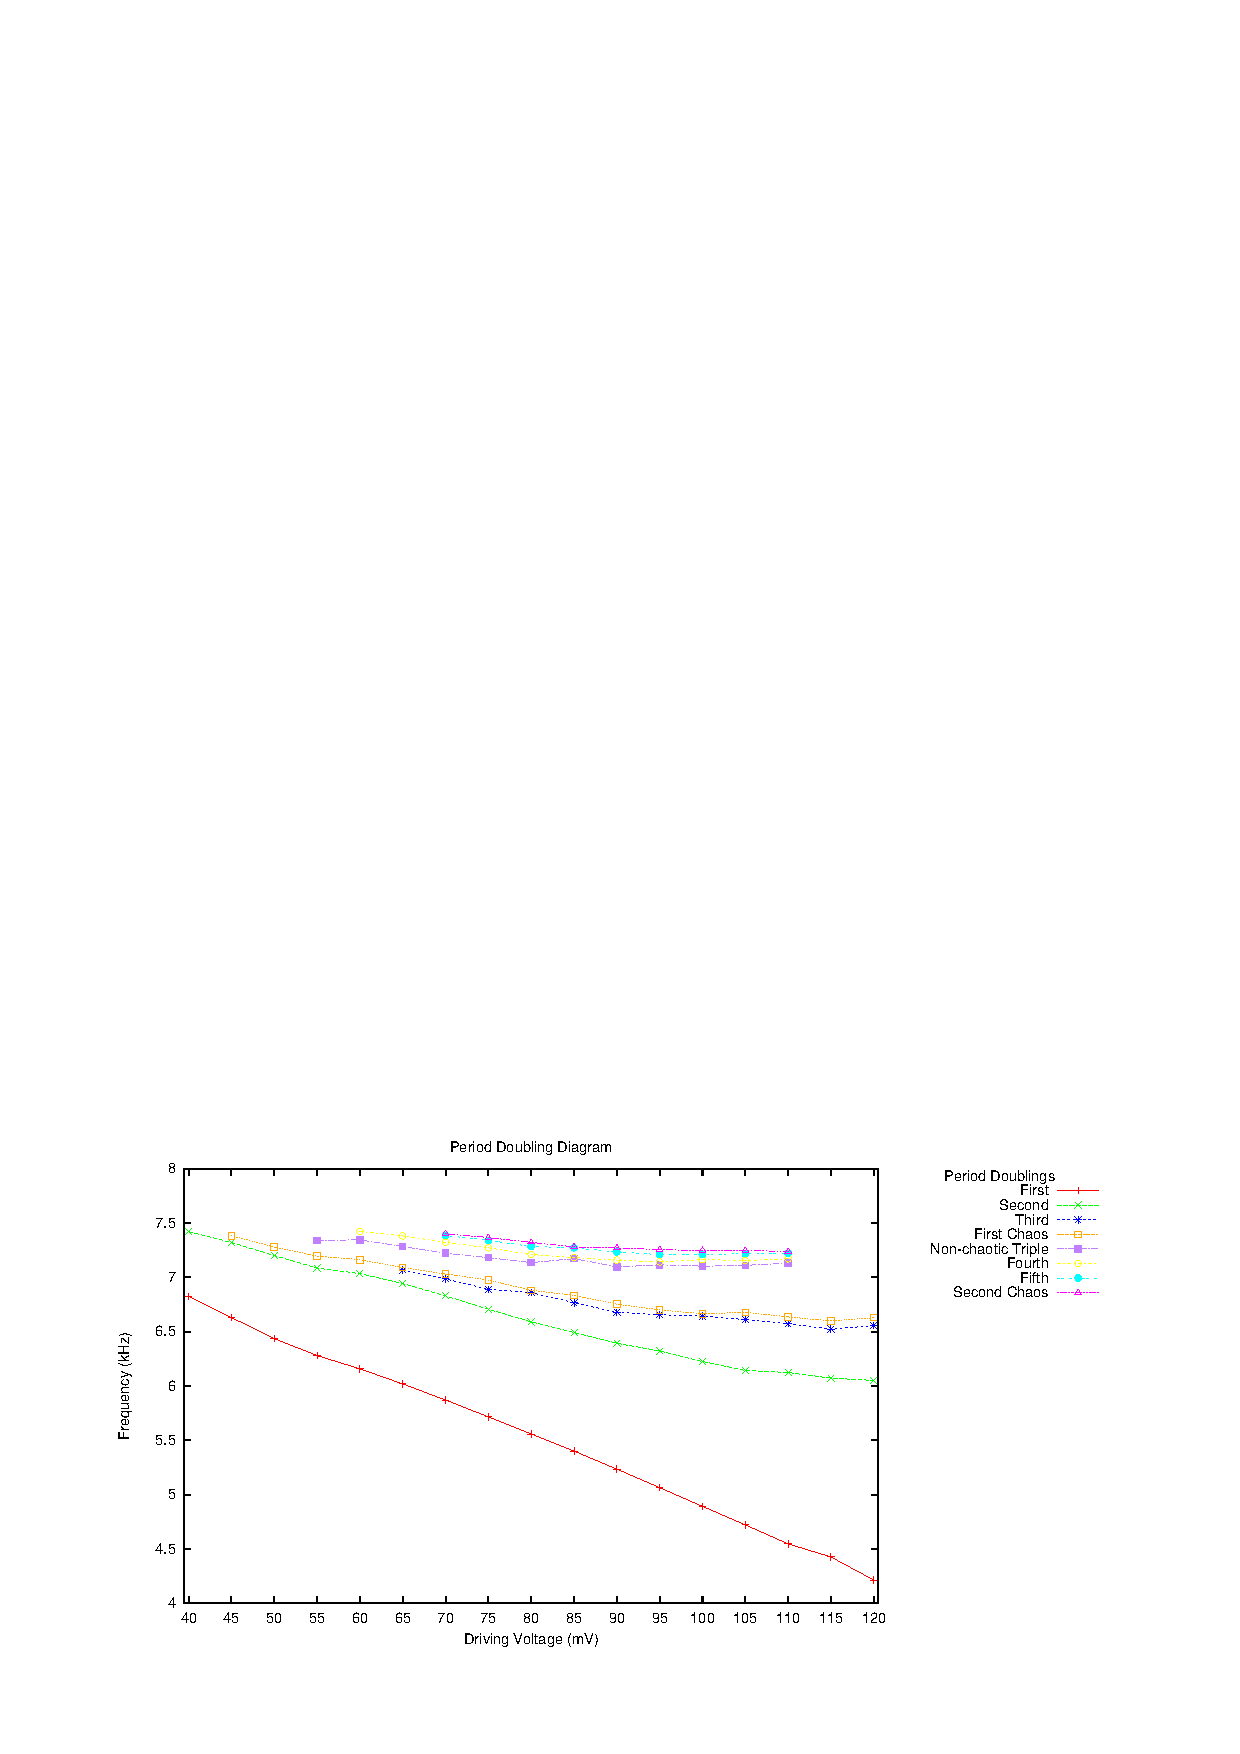
\includegraphics{plots/general.pdf}
		\label{fig:periodDoubling}
		\caption{Period Doubling}
	\end{figure}

	\begin{figure}[h]
		\centering
		\includegraphics{simulations/circuit.png}
	\end{figure}

	\begin{table}
		\centering
		\begin{tabular}{|l|l|l||l|l|l|}
			\hline
			Vdrive (V) & Vdrive error & Vresistor (mV)   \\ \hline
12.5 & 0.1 & 63.5                            \\ \hline
13.3 & 0.1 & 68                              \\ \hline
13.6 & 0.1 & 70                              \\ \hline
14.2 & 0.1 & 72                              \\ \hline
14.6 & 0.1 & 74                              \\ \hline
15.3 & 0.1 & 77                              \\ \hline
16.1 & 0.1 & 80.5                            \\ \hline
17.1 & 0.1 & 84                              \\ \hline
17.3 & 0.1 & 84.5                            \\ \hline
17.5 & 0.1 & 87.5                            \\ \hline
17.5 &  & 82.5                               \\ \hline
17.8 & 0.1 & 89.5                            \\ \hline
17.8 &  & 81                                 \\ \hline
18.1 & 0.1 & 92.5                            \\ \hline
18.1 &  & 77                                 \\ \hline
18.5 & 0.1 & 94                              \\ \hline
18.5 &  & 75                                 \\ \hline
18.9 & 0.1 & 96.5                            \\ \hline
18.9 &  & 73                                 \\ \hline
19.3 & 0.1 & 100                             \\ \hline
19.3 &  & 70.5                               \\ \hline
19.9 & 0.1 & 105.5                           \\ \hline
19.9 &  & 69.5                               \\ \hline
20.7 & 0.1 & 71.5                            \\ \hline
20.7 &  & 112                                \\ \hline
21.1 & 0.1 & 115                             \\ \hline
21.1 &  & 72.5                               \\ \hline
21.2 & 0.1 & 117                             \\ \hline
21.2 &  & 114                                \\ \hline
21.2 &  & 76.5                               \\ \hline
21.2 &  & 70.5                               \\ \hline
21.3 & 0.1 & 119                             \\ \hline
21.3 &  & 112.5                              \\ \hline
21.3 &  & 73                                 \\ \hline
21.3 &  & 75                                 \\ \hline
21.4 & 0.1 & 120.5                           \\ \hline
21.4 &  & 112                                \\ \hline
21.4 &  & 77.5                               \\ \hline
21.4 &  & 73.5                               \\ \hline
21.5 & 0.1 & 121                             \\ \hline
21.5 &  & 112                                \\ \hline
21.5 &  & 74                                 \\ \hline
21.5 &  & 79                                 \\ \hline
21.6 & 0.1 & 122                             \\ \hline
21.6 &  & 120.5                              \\ \hline
21.6 &  & 114.5                              \\ \hline
21.6 &  & 112                                \\ \hline
21.6 &  & 80                                 \\ \hline
21.6 &  & 79                                 \\ \hline
21.6 &  & 73                                 \\ \hline
21.6 &  & 73.5                               \\ \hline
21.7 &  & CHAOS                              \\ \hline
22.3 & 0.1 & 76.5                            \\ \hline
22.3 &  & 81                                 \\ \hline
22.3 &  & 137                                \\ \hline
22.5 & 0.1 & 77.5                            \\ \hline
22.5 &  & 81.5                               \\ \hline
22.5 &  & 140                                \\ \hline
22.6 & 0.1 & 82.5                            \\ \hline
22.6 &  & 72.5                               \\ \hline
22.6 &  & 81                                 \\ \hline
22.6 &  & 83.5                               \\ \hline
22.6 &  & 141                                \\ \hline
22.6 &  & 138                                \\ \hline
22.7 & 0.1 & Chaos                           \\ \hline
 
		\end{tabular}
		\label{tab:80khz}
		\caption{Data for Bifurcation plot, 80 kHz}
	\end{table}

	\begin{table}
		\centering
		\begin{tabular}{|l|l|l|l||l|l|l|l|}
			\hline
			V$_{\rm drive}$ (V) & $\sigma_{\rm V_{\rm drive}}$ & V$_{\rm R}$ (mV) & $\sigma_{\rm V_{\rm R}}$ &V$_{\rm drive}$ (V) & $\sigma_{\rm V_{\rm drive}}$ & V$_{\rm R}$ (mV) & $\sigma_{\rm V_{\rm R}}$       \\ \hline
14.5 & 0.1 & 55.5 & 5                                     &  20.8 & 0.1 & 92.5 &                                    \\ \hline
14.9 & 0.1 & 58 & 5                                       &  20.8 &  & 86.5 &                                       \\ \hline
15.3 & 0.1 & 59 & 5                                       &  20.8 &  & 57 &                                         \\ \hline
15.7 & 0.1 & 61.5 & 5                                     &  20.8 &  & 61 &                                         \\ \hline
15.7 &  & 57 &                                            &  21.1 & 0.1 & 93 &                                      \\ \hline
16.1 & 0.1 & 64.5 &                                       &  21.1 &  & 91.5 &                                       \\ \hline
16.1 &  & 55 &                                            &  21.1 &  & 88.5 &                                       \\ \hline
16.7 & 0.1 & 68.5 &                                       &  21.1 &  & 85.5 &                                       \\ \hline
16.7 &  & 52.5 &                                          &  21.1 &  & 64 &                                         \\ \hline
17.1 & 0.1 & 71 &                                         &  21.1 &  & 61 &                                         \\ \hline
17.1 &  & 51.5 &                                          &  21.1 &  & 56.5 &                                       \\ \hline
17.5 & 0.1 & 73.5 &                                       &  21.1 &  & 55.5 &                                       \\ \hline
17.5 &  & 50.5 &                                          &  21.2 &  & CHAOS &                                      \\ \hline
18.1 & 0.1 & 77 &                                         &  22.1 & 0.1 & 61 &                                      \\ \hline
18.1 &  & 50.5 &                                          &  22.1 &  & 76.5 &                                       \\ \hline
18.7 & 0.1 & 50.5 &                                       &  22.1 &  & 95 &                                         \\ \hline
18.7 &  & 80 &                                            &  22.3 & 0.1 & 110 &                                     \\ \hline
19.5 & 0.1 & 85.5 &                                       &  22.3 &  & 108.5 &                                      \\ \hline
19.5 &  & 54 &                                            &  22.3 &  & 64 &                                         \\ \hline
19.9 & 0.1 & 86.5 &                                       &  22.3 &  & 66 &                                         \\ \hline
19.9 &  & 54.5 &                                          &  22.3 &  & 65 &                                         \\ \hline
20.3 & 0.1 & 88.5 &                                       &  22.3 &  & 57 &                                         \\ \hline
20.3 &  & 86 &                                            &  22.5 &  & CHAOS &                                      \\ \hline
20.3 &  & 54 &                                                                                                      \\ \cline{1-4}
20.3 &  & 55.5 &                                                                                                    \\ \cline{1-4}
20.5 & 0.1 & 90 &                                                                                                   \\ \cline{1-4}
20.5 &  & 86.5 &                                                                                                    \\ \cline{1-4}
20.5 &  & 59 &                                                                                                      \\ \cline{1-4}
20.5 &  & 54.5 &                                                                                                    \\ \cline{1-4}
                                  
                                  
                                  
                                  
                                  
                                  
                                  
                                  
                                  
                                  
                                  
                                  
                                  
                                  
                                  
                                  
                                  
                                  
                                  
                                  
                                  
                                  
                                  
 
		\end{tabular}
		\label{tab:100khz}
		\caption{Data for Bifurcation plot, 100 kHz}
	\end{table}

    %\pagebreak

	\begin{table}
		\centering
		\begin{tabular}{|c|c|c|c|c|}
			\hline
			Test & $\bar\delta$ & $\sigma_{\bar\delta}$ & $\bar\alpha$ & $\sigma_{\bar\alpha}$                 \\ \hline
\multirow{4}{*}{80 kHz} & 4.866354752 & 0.587017407 & 5.00952381 & 5.677672139        \\\cline{2-5} 
 & 5.071945093 & 3.588190355 & 5.96026196 & 7.723440964              \\ \cline{2-5} 
 &  &  & 31 & 151.037876                                             \\ \cline{2-5} 
 &  &  & 8.818145743 & 14.47253609                                   \\ \hline\hline
 \multirow{4}{*}{120 kHz} & 3.970268152 & 0.233369321 & 7.617629429 & 20.52787139      \\ \cline{2-5} 
 & 6.332809588 & 3.635471291 & 9.867676768 & 31.02307017             \\ \cline{2-5} 
 &  &  & 26.12619048 & 247.3949034                                   \\ \cline{2-5} 
 &  &  & 7.404079254 & 14.37760074                                   \\ \hline \hline
10.444 V & 4.664396154 & 0.761125658 &  &                            \\ \hline
 
		\end{tabular}
		\label{tab:fegeinbaum}
		\caption{Stuff}
	\end{table}

	\begin{table}
		\centering
		\begin{tabular}{|c|c|c|c|c|}
			\hline
			V$_{\rm drive}$ (mV) & Frequency (kHz) & Freq. error & $\delta$ & $\sigma_{\delta}$   \\ \hline
10443.96716 & 24.15 & 0.22 & 4.958188153 & 1.876232418              \\ \hline
 & 38.38 & 0.69 &  &                                                \\ \hline
 & 41.25 & 0.7 &  &                                                 \\ \hline
 & 24.14 & 0.22 & 4.283076923 & 1.453848818                         \\ \hline
 & 38.06 & 0.69 &  &                                                \\ \hline
 & 41.31 & 0.7 &  &                                                 \\ \hline
 & 24.13 & 0.22 & 4.815068493 & 1.796177384                         \\ \hline
 & 38.19 & 0.69 &  &                                                \\ \hline
 & 41.11 & 0.7 &  &                                                 \\ \hline
 & 24.07 & 0.22 & 4.728187919 & 1.731510497                         \\ \hline
 & 38.16 & 0.69 &  &                                                \\ \hline
 & 41.14 & 0.7 &  &                                                 \\ \hline
 & 24.15 & 0.22 & 4.537459283 & 1.620030996                         \\ \hline
 & 38.08 & 0.69 &  &                                                \\ \hline
 & 41.15 & 0.7 &  &                                                 \\ \hline
 
		\end{tabular}
		\label{tab:chaos3}
		\caption{Some data}
	\end{table}

	\begin{table}
		\centering
		\begin{tabular}{|l|l|l|l|l|l|l|l|l|l|l|l|}
			\hline
			Frequency (kHz) & Freq error & V drive (mV) & Vd tot error & Vresistor (mV) & Vr tot error & Vr difference & Diff error & DELTA & DELTA ERROR & ALPHA & ALPHA ERR    \\ \hline
80 & 0.1 & 7884.24061 & 23.79898987 & 89 & 6 &  &  & 4.747706422 & 1.258301434 & 4.666666667 & 9.778989824                                                           \\ \hline
 &  & 9347.951647 & 46.01219331 & 117.5 & 7 & 44.5 & 9.899494937 & 5.891891892 & 9.648282024 & 6.363636364 & 17.60959807                                             \\ \hline
 &  &  &  & 73 &  &  &  &  &  & DIV/0! & DIV/0!                                                                                                                    \\ \hline
 &  & 9656.250204 & 59.56854249 & 123 & 7 & 9.5 & 9.899494937 &  &  & 8.777777778 & 28.98967331                                                                      \\ \hline
 &  &  &  & 113.5 &  &  &  &  &  &  &                                                                                                                                \\ \hline
 &  &  &  & 79.5 &  & 5 &  &  &  &  &                                                                                                                                \\ \hline
 &  &  &  & 74.5 &  &  &  &  &  &  &                                                                                                                                 \\ \hline
 &  & 9708.576106 & 49.254834 & 124.5 & 7 & 2 & 9.899494937 &  &  &  &                                                                                               \\ \hline
 &  &  &  & 122.5 &  &  &  &  &  &  &                                                                                                                                \\ \hline
 &  &  &  & 116 &  & 4 &  &  &  &  &                                                                                                                                 \\ \hline
 &  &  &  & 112 &  &  &  &  &  &  &                                                                                                                                  \\ \hline
 &  &  &  & 83.5 &  & 5 &  &  &  &  &                                                                                                                                \\ \hline
 &  &  &  & 78.5 &  &  &  &  &  &  &                                                                                                                                 \\ \hline
 &  &  &  & 75 &  & 0.5 &  &  &  &  &                                                                                                                                \\ \hline
 &  &  &  & 75.5 &  &  &  &  &  &  &                                                                                                                                 \\ \hline\hline
79.6 & 0.1 & 7854.542125 & 22.79898987 & 87 & 6 &  &  & 4.764976959 & 1.266868276 & 4.466666667 & 9.410995408                                                        \\ \hline
 &  & 9316.838949 & 45.01219331 & 117 & 7 & 43 & 9.899494937 & 4.34 & 5.486277344 & 6.090909091 & 16.92106731                                                        \\ \hline
 &  &  &  & 74 &  &  &  &  &  & DIV/0! & DIV/0!                                                                                                                    \\ \hline
 &  & 9623.723292 & 60.56854249 & 123 & 7 & 9.5 & 9.899494937 &  &  & 8.444444444 & 27.95729101                                                                      \\ \hline
 &  &  &  & 113.5 &  &  &  &  &  &  &                                                                                                                                \\ \hline
 &  &  &  & 80 &  & 5 &  &  &  &  &                                                                                                                                  \\ \hline
 &  &  &  & 75 &  &  &  &  &  &  &                                                                                                                                   \\ \hline
 &  & 9694.43397 & 48.254834 & 125 & 7 & 2 & 9.899494937 &  &  &  &                                                                                                  \\ \hline
 &  &  &  & 123 &  &  &  &  &  &  &                                                                                                                                  \\ \hline
 &  &  &  & 116.5 &  & 4 &  &  &  &  &                                                                                                                               \\ \hline
 &  &  &  & 112.5 &  &  &  &  &  &  &                                                                                                                                \\ \hline
 &  &  &  & 84 &  & 5 &  &  &  &  &                                                                                                                                  \\ \hline
 &  &  &  & 79 &  &  &  &  &  &  &                                                                                                                                   \\ \hline
 &  &  &  & 75 &  & 0.5 &  &  &  &  &                                                                                                                                \\ \hline
 &  &  &  & 75.5 &  &  &  &  &  &  &                                                                                                                                 \\ \hline\hline
80 & 0.1 & 7855.956339 & 21.79898987 & 87 & 6 &  &  & 4.933333333 & 1.351438088 & 4.4 & 9.288425294                                                                  \\ \hline
 &  & 9321.08159 & 45.01219331 & 117 & 7 & 42.5 & 9.899494937 & 5.12195122 & 7.724520182 & 4.714285714 & 10.57142857                                                 \\ \hline
 &  &  &  & 74.5 &  &  &  &  &  & 36.5 & 518.1418725                                                                                                                 \\ \hline
 &  & 9618.066438 & 60.56854249 & 123 & 7 & 9.5 & 9.899494937 &  &  & 6.636363636 & 18.29855836                                                                      \\ \hline
 &  &  &  & 113.5 &  &  &  &  &  &  &                                                                                                                                \\ \hline
 &  &  &  & 81 &  & 6 &  &  &  &  &                                                                                                                                  \\ \hline
 &  &  &  & 75 &  &  &  &  &  &  &                                                                                                                                   \\ \hline
 &  & 9676.049194 & 48.254834 & 124 & 7 & 2 & 9.899494937 &  &  &  &                                                                                                 \\ \hline
 &  &  &  & 122 &  &  &  &  &  &  &                                                                                                                                  \\ \hline
 &  &  &  & 115 &  & 2.5 &  &  &  &  &                                                                                                                               \\ \hline
 &  &  &  & 112.5 &  &  &  &  &  &  &                                                                                                                                \\ \hline
 &  &  &  & 83.5 &  & 5 &  &  &  &  &                                                                                                                                \\ \hline
 &  &  &  & 78.5 &  &  &  &  &  &  &                                                                                                                                 \\ \hline
 &  &  &  & 75 &  & 0.5 &  &  &  &  &                                                                                                                                \\ \hline
 &  &  &  & 74.5 &  &  &  &  &  &  &                                                                                                                                 \\ \hline\hline
80 & 0.1 & 7831.914708 & 22.79898987 & 86.5 & 6 &  &  & 4.938388626 & 1.347657981 & 6.8 & 20.58333306                                                                \\ \hline
 &  & 9305.52524 & 46.01219331 & 116 & 7 & 42 & 9.899494937 & 6.205882353 & 10.92689684 & 7.555555556 & 25.20613991                                                  \\ \hline
 &  &  &  & 74 &  &  &  &  &  & 19 & 136.6345491                                                                                                                     \\ \hline
 &  & 9603.924302 & 59.56854249 & 121.5 & 7 & 8 & 9.899494937 &  &  & 10.85714286 & 45.56045546                                                                      \\ \hline
 &  &  &  & 113.5 &  &  &  &  &  &  &                                                                                                                                \\ \hline
 &  &  &  & 79 &  & 4 &  &  &  &  &                                                                                                                                  \\ \hline
 &  &  &  & 75 &  &  &  &  &  &  &                                                                                                                                   \\ \hline
 &  & 9652.007563 & 48.254834 & 123.5 & 7 & 3 & 9.899494937 &  &  &  &                                                                                               \\ \hline
 &  &  &  & 120.5 &  &  &  &  &  &  &                                                                                                                                \\ \hline
 &  &  &  & 115.5 &  & 3.5 &  &  &  &  &                                                                                                                             \\ \hline
 &  &  &  & 112 &  &  &  &  &  &  &                                                                                                                                  \\ \hline
 &  &  &  & 83 &  & 2 &  &  &  &  &                                                                                                                                  \\ \hline
 &  &  &  & 81 &  &  &  &  &  &  &                                                                                                                                   \\ \hline
 &  &  &  & 74.5 &  & 0.5 &  &  &  &  &                                                                                                                              \\ \hline
 &  &  &  & 75 &  &  &  &  &  &  &                                                                                                                                   \\ \hline
 &  &  &  &  &  &  &  &  &  &  &                                                                                                                                     \\ \hline
80 & 0.1 & 7823.429427 & 21.79898987 & 86.5 & 6 &  &  & 4.947368421 & 1.335623916 & 4.714285714 & 10.57142857                                                        \\ \hline
 &  & 9285.726251 & 44.01219331 & 115.5 & 7 & 42.5 & 9.899494937 & 3.8 & 4.429884742 & 5.076923077 & 12.15579918                                                     \\ \hline
 &  &  &  & 73 &  &  &  &  &  & 37.5 & 532.13814                                                                                                                     \\ \hline
 &  & 9581.296885 & 59.56854249 & 121.5 & 7 & 9.5 & 9.899494937 &  &  & 9.375 & 34.69515681                                                                          \\ \hline
 &  &  &  & 112 &  &  &  &  &  &  &                                                                                                                                  \\ \hline
 &  &  &  & 79 &  & 5 &  &  &  &  &                                                                                                                                  \\ \hline
 &  &  &  & 74 &  &  &  &  &  &  &                                                                                                                                   \\ \hline
 &  & 9659.078631 & 49.254834 & 123 & 7 & 2.5 & 9.899494937 &  &  &  &                                                                                               \\ \hline
 &  &  &  & 120.5 &  &  &  &  &  &  &                                                                                                                                \\ \hline
 &  &  &  & 114.5 &  & 3 &  &  &  &  &                                                                                                                               \\ \hline
 &  &  &  & 111.5 &  &  &  &  &  &  &                                                                                                                                \\ \hline
 &  &  &  & 83.5 &  & 4 &  &  &  &  &                                                                                                                                \\ \hline
 &  &  &  & 79.5 &  &  &  &  &  &  &                                                                                                                                 \\ \hline
 &  &  &  & 74 &  & 1 &  &  &  &  &                                                                                                                                  \\ \hline
 &  &  &  & 75 &  &  &  &  &  &  &                                                                                                                                   \\ \hline
 &  &  &  &  &  &  &  &  &  &  &                                                                                                                                     \\ \hline
120 & 0.1 & 6040.106125 & 37.35533906 & 48 & 7 &  &  & 3.959910913 & 0.513624498 & 6.538461538 & 26.18414802                                                         \\ \hline
 &  & 8554.577839 & 44.42640687 & 71 & 6 & 25.75 & 8.485281374 & 7.877192982 & 10.87821271 & 7.727272727 & 36.09917355                                               \\ \hline
 &  &  &  & 45.25 &  &  &  &  &  & 29.66666667 & 482.8655207                                                                                                         \\ \hline
 &  & 9189.559728 & 59.98275606 & 75.25 & 6 & 4.5 & 8.485281374 &  &  & 7.416666667 & 31.85557687                                                                    \\ \hline
 &  &  &  & 70.75 &  &  &  &  &  &  &                                                                                                                                \\ \hline
 &  &  &  & 50.25 &  & 3.5 &  &  &  &  &                                                                                                                             \\ \hline
 &  &  &  & 46.75 &  &  &  &  &  &  &                                                                                                                                \\ \hline
 &  & 9270.169901 & 88.2670273 & 76 & 6 & 1.25 & 8.485281374 &  &  &  &                                                                                              \\ \hline
 &  &  &  & 74.75 &  &  &  &  &  &  &                                                                                                                                \\ \hline
 &  &  &  & 72 &  & 1.75 &  &  &  &  &                                                                                                                               \\ \hline
 &  &  &  & 70.25 &  &  &  &  &  &  &                                                                                                                                \\ \hline
 &  &  &  & 52 &  & 2.75 &  &  &  &  &                                                                                                                               \\ \hline
 &  &  &  & 49.25 &  &  &  &  &  &  &                                                                                                                                \\ \hline
 &  &  &  & 47 &  & 0.5 &  &  &  &  &                                                                                                                                \\ \hline
 &  &  &  & 47.5 &  &  &  &  &  &  &                                                                                                                                 \\ \hline
 &  &  &  &  &  &  &  &  &  &  &                                                                                                                                     \\ \hline
120 & 0.1 & 6055.662474 & 37.35533906 & 48 & 7 &  &  & 4.002257336 & 0.52556325 & 7.909090909 & 36.88829621                                                          \\ \hline
 &  & 8563.06312 & 44.42640687 & 71.25 & 6 & 26 & 8.485281374 & 5.273809524 & 5.052756239 & 14.5 & 120.1998336                                                       \\ \hline
 &  &  &  & 45.25 &  &  &  &  &  & 22.25 & 273.1977306                                                                                                               \\ \hline
 &  & 9189.559728 & 59.98275606 & 75 & 6 & 4.25 & 8.485281374 &  &  & 6.846153846 & 27.31209168                                                                      \\ \hline
 &  &  &  & 70.75 &  &  &  &  &  &  &                                                                                                                                \\ \hline
 &  &  &  & 50.5 &  & 3.75 &  &  &  &  &                                                                                                                             \\ \hline
 &  &  &  & 46.75 &  &  &  &  &  &  &                                                                                                                                \\ \hline
 &  & 9308.353668 & 88.2670273 & 76.5 & 6 & 1.5 & 8.485281374 &  &  &  &                                                                                             \\ \hline
 &  &  &  & 75 &  &  &  &  &  &  &                                                                                                                                   \\ \hline
 &  &  &  & 72.5 &  & 2.75 &  &  &  &  &                                                                                                                             \\ \hline
 &  &  &  & 69.75 &  &  &  &  &  &  &                                                                                                                                \\ \hline
 &  &  &  & 52.5 &  & 2.75 &  &  &  &  &                                                                                                                             \\ \hline
 &  &  &  & 49.75 &  &  &  &  &  &  &                                                                                                                                \\ \hline
 &  &  &  & 47 &  & 0.5 &  &  &  &  &                                                                                                                                \\ \hline
 &  &  &  & 47.5 &  &  &  &  &  &  &                                                                                                                                 \\ \hline
 &  &  &  &  &  &  &  &  &  &  &                                                                                                                                     \\ \hline
120 & 0.1 & 6050.00562 & 37.35533906 & 48 & 7 &  &  & 3.800429185 & 0.477060374 & 4.882352941 & 15.39269613                                                          \\ \hline
 &  & 8554.577839 & 44.42640687 & 70.75 & 6 & 25.5 & 8.485281374 & 8.175438596 & 11.2719576 & 6.916666667 & 29.86822913                                              \\ \hline
 &  &  &  & 45.25 &  &  &  &  &  & 44 & 1068.202228                                                                                                                  \\ \hline
 &  & 9213.601359 & 59.98275606 & 75.25 & 6 & 4.75 & 8.485281374 &  &  & 7.333333333 & 31.52424111                                                                   \\ \hline
 &  &  &  & 70.5 &  &  &  &  &  &  &                                                                                                                                 \\ \hline
 &  &  &  & 50.5 &  & 3.5 &  &  &  &  &                                                                                                                              \\ \hline
 &  &  &  & 47 &  &  &  &  &  &  &                                                                                                                                   \\ \hline
 &  & 9294.211532 & 88.2670273 & 75.5 & 6 & 0.5 & 8.485281374 &  &  &  &                                                                                             \\ \hline
 &  &  &  & 75 &  &  &  &  &  &  &                                                                                                                                   \\ \hline
 &  &  &  & 72 &  & 1.75 &  &  &  &  &                                                                                                                               \\ \hline
 &  &  &  & 70.25 &  &  &  &  &  &  &                                                                                                                                \\ \hline
 &  &  &  & 52.5 &  & 3 &  &  &  &  &                                                                                                                                \\ \hline
 &  &  &  & 49.5 &  &  &  &  &  &  &                                                                                                                                 \\ \hline
 &  &  &  & 47.5 &  & 0.5 &  &  &  &  &                                                                                                                              \\ \hline
 &  &  &  & 48 &  &  &  &  &  &  &                                                                                                                                   \\ \hline
 &  &  &  &  &  &  &  &  &  &  &                                                                                                                                     \\ \hline
120 & 0.1 & 6051.419833 & 37.35533906 & 48.25 & 7 &  &  & 4.137850467 & 0.565523271 & 6.615384615 & 26.46606856                                                      \\ \hline
 &  & 8555.992052 & 44.42640687 & 70.75 & 6 & 25.5 & 8.485281374 & 4.115384615 & 3.290696101 & 10.75 & 67.69970458                                                   \\ \hline
 &  &  &  & 45.25 &  &  &  &  &  & 12.71428571 & 90.80663099                                                                                                         \\ \hline
 &  & 9161.275457 & 60.98275606 & 74.75 & 6 & 4 & 8.485281374 &  &  & 8.090909091 & 37.67759803                                                                      \\ \hline
 &  &  &  & 70.75 &  &  &  &  &  &  &                                                                                                                                \\ \hline
 &  &  &  & 46.75 &  & 3.25 &  &  &  &  &                                                                                                                            \\ \hline
 &  &  &  & 50 &  &  &  &  &  &  &                                                                                                                                   \\ \hline
 &  & 9308.353668 & 89.2670273 & 75.5 & 6 & 0.75 & 8.485281374 &  &  &  &                                                                                            \\ \hline
 &  &  &  & 74.75 &  &  &  &  &  &  &                                                                                                                                \\ \hline
 &  &  &  & 72.25 &  & 2 &  &  &  &  &                                                                                                                               \\ \hline
 &  &  &  & 70.25 &  &  &  &  &  &  &                                                                                                                                \\ \hline
 &  &  &  & 52.5 &  & 1.5 &  &  &  &  &                                                                                                                              \\ \hline
 &  &  &  & 51 &  &  &  &  &  &  &                                                                                                                                   \\ \hline
 &  &  &  & 47.25 &  & 0.5 &  &  &  &  &                                                                                                                             \\ \hline
 &  &  &  & 47.75 &  &  &  &  &  &  &                                                                                                                                \\ \hline
 &  &  &  &  &  &  &  &  &  &  &                                                                                                                                     \\ \hline
120 & 0.1 & 6059.905115 & 37.35533906 & 48 & 7 &  &  & 3.950892857 & 0.52354653 & 12.14285714 & 86.89702936                                                          \\ \hline
 &  & 8563.06312 & 45.42640687 & 70.75 & 6 & 25.5 & 8.485281374 & 6.222222222 & 6.976010433 & 9.444444444 & 53.23777447                                              \\ \hline
 &  &  &  & 45.25 &  &  &  &  &  & 22 & 270.199926                                                                                                                   \\ \hline
 &  & 9196.630796 & 60.98275606 & 75 & 6 & 4.25 & 8.485281374 &  &  & 7.333333333 & 31.52424111                                                                      \\ \hline
 &  &  &  & 70.75 &  &  &  &  &  &  &                                                                                                                                \\ \hline
 &  &  &  & 50.25 &  & 3.5 &  &  &  &  &                                                                                                                             \\ \hline
 &  &  &  & 46.75 &  &  &  &  &  &  &                                                                                                                                \\ \hline
 &  & 9298.454173 & 89.2670273 & 76 & 6 & 2.5 & 8.485281374 &  &  &  &                                                                                               \\ \hline
 &  &  &  & 74.75 &  &  &  &  &  &  &                                                                                                                                \\ \hline
 &  &  &  & 72.25 &  & 2 &  &  &  &  &                                                                                                                               \\ \hline
 &  &  &  & 70.25 &  &  &  &  &  &  &                                                                                                                                \\ \hline
 &  &  &  & 52.25 &  & 2.5 &  &  &  &  &                                                                                                                             \\ \hline
 &  &  &  & 49.75 &  &  &  &  &  &  &                                                                                                                                \\ \hline
 &  &  &  & 47 &  & 0.5 &  &  &  &  &                                                                                                                                \\ \hline
 &  &  &  & 47.5 &  &  &  &  &  &  &                                                                                                                                 \\ \hline
 
		\end{tabular}
		\label{tab:chaos2}
		\caption{Some more data}
	\end{table}

\chapter*{Appendix}

	\end{document}

